\documentclass[aspectratio=43, xcolor=table]{beamer}
%\usepackage[english]{babel}

%Cargar paquetes
\usepackage[utf8]{inputenc}%Permite usar acentos
\usepackage[spanish]{babel}%Configura el idioma por defecto a español
\usepackage{amsmath}%Introduce términos matemáticos
\usepackage{graphicx}%Permite introducir figuras
\usepackage[options]{natbib}%Bibliografía con estilos %No funcionan estilos en Beamer
\newcommand{\grad}{\hspace{-2mm}$\phantom{a}^{\circ}$}

\usepackage{amsthm}
\usepackage{mathtools}
\usepackage{physics}
\usepackage{calligra}
\usepackage{csquotes}
\usepackage{tensor}
\usepackage[thicklines]{cancel}
\usepackage{tcolorbox}
\usepackage{pstricks}
\usepackage[backend=biber, bibstyle=nature, sorting=nty, citestyle=numeric-comp]{biblatex} %Custom bibliography
    \addbibresource{bib.bib} %Load references


\DeclareMathAlphabet{\mathcalligra}{T1}{calligra}{m}{n}
\DeclareFontShape{T1}{calligra}{m}{n}{<->s*[2.2]callig15}{}
\newcommand{\scriptr}{\mathcalligra{r}\,}
\newcommand{\boldscriptr}{\pmb{\mathcalligra{r}}\,}
\def\rc{\scriptr}
\def\brc{\boldscriptr}
\def\hrc{\hat\brc}
\newcommand{\ie}{\emph{i.e.}} %id est
\newcommand{\eg}{\emph{e.g.}} %exempli gratia
\newcommand{\rtd}[1]{\ensuremath{\left\lfloor #1 \right\rfloor}}
\newcommand{\dirac}[1]{\ensuremath{\delta \left( #1 \right)}}
\newcommand{\diract}[1]{\ensuremath{\delta^3 \left( #1 \right)}}
\newcommand{\e}{\ensuremath{\epsilon_0}}
\newcommand{\m}{\ensuremath{\mu_0}}
\newcommand{\V}{\ensuremath{\mathcal{V}}}
\newcommand{\prnt}[1]{\ensuremath{\left(#1\right)}} %parentheses
\newcommand{\colch}[1]{\ensuremath{\left[#1\right]}} %square brackets
\newcommand{\chave}[1]{\ensuremath{\left\{#1\right\}}}  %curly brackets

\useoutertheme{infolines}
\useinnertheme{rectangles}
\usefonttheme{professionalfonts}


\definecolor{orange}{HTML}{f28165}
\definecolor{gray}{HTML}{303030}
\definecolor{yellow}{HTML}{f0be52}
\definecolor{lightorange}{HTML}{f19e58}

\renewcommand{\CancelColor}{\color{orange}}

\makeatletter
\newcommand{\mybox}[1]{%
  \setbox0=\hbox{#1}%
  \setlength{\@tempdima}{\dimexpr\wd0+13pt}%
  \begin{tcolorbox}[colback=orange,colframe=orange,boxrule=0.5pt,arc=4pt,
      left=6pt,right=6pt,top=6pt,bottom=6pt,boxsep=0pt,width=\@tempdima]
    \textcolor{white}{#1}
  \end{tcolorbox}
}
\makeatother

\usecolortheme[named=orange]{structure}
\usecolortheme{sidebartab}
\usecolortheme{orchid}
\usecolortheme{whale}
\setbeamercolor{alerted text}{fg=yellow}
\setbeamercolor{block title alerted}{bg=alerted text.fg!90!black}
\setbeamercolor{block title example}{bg=lightorange!60!black}
\setbeamercolor{background canvas}{bg=gray}
\setbeamercolor{normal text}{bg=gray,fg=white}

\setbeamertemplate{footline}
        {
      \leavevmode%
      \hbox{%
      \begin{beamercolorbox}[wd=.333333\paperwidth,ht=2.25ex,dp=1ex,center]{author in head/foot}%
        \usebeamerfont{author in head/foot}\insertshortauthor~~(\insertshortinstitute)
      \end{beamercolorbox}%
      \begin{beamercolorbox}[wd=.333333\paperwidth,ht=2.25ex,dp=1ex,center]{title in head/foot}%
        \usebeamerfont{title in head/foot}\insertshorttitle
      \end{beamercolorbox}%
      \begin{beamercolorbox}[wd=.333333\paperwidth,ht=2.25ex,dp=1ex,center]{date in head/foot}%
        \usebeamerfont{page number in head/foot}\insertframenumber/\inserttotalframenumber%\hspace*{2em}

    %#turning the next line into a comment, erases the frame numbers
        %\insertframenumber{} / \inserttotalframenumber\hspace*{2ex} 

      \end{beamercolorbox}}%
      \vskip0pt%
    }


\setbeamertemplate{blocks}[rectangle]
\setbeamercovered{dynamic}

\setbeamertemplate{section page}
{
	\begin{centering}
		\begin{beamercolorbox}[sep=27pt,center]{part title}
			\usebeamerfont{section title}\insertsection\par
			\usebeamerfont{subsection title}\insertsubsection\par
		\end{beamercolorbox}
	\end{centering}
}

%\setbeamertemplate{subsection page}
%{
%	\begin{centering}
%		\begin{beamercolorbox}[sep=12pt,center]{part title}
%			\usebeamerfont{subsection title}\insertsubsection\par
%		\end{beamercolorbox}
%	\end{centering}
%}

\newcommand{\hlight}[1]{\colorbox{violet!50}{#1}}
\newcommand{\hlighta}[1]{\colorbox{red!50}{#1}}
\title{Generación de variables aleatorias} %->->->->-> Check hyperref title <-<-<-<-<-
%\subtitle{And Some Things About It}
\author[C.J. Uribe-Martes]{Carlos Javier Uribe Martes}
\institute[CUC]{
    Ingeniería Industrial%
    \\%
    Universidad de la Costa%
} %You can change the Institution if you are from somewhere else
\date{Febrero 12, 2020}
%\logo{\includegraphics[width= 0.2\textwidth]{images/a-logo.png}}

\begin{document}
    
    \frame{\titlepage}
    
    %\section{Introducción}

\begin{frame}{Generación de variables aleatorias}
    \begin{itemize}
        \item Los modelos de simulación usualmente contienen actividades o atributos cuya duración o valor es impredecible o incierto.
        \item Para modelar este tipo de situaciones es útil emplear \textit{variables aleatorias} con distribuciones de probabilidad específicas.
        %\item Las variables aleatorias se pueden clasificar en variables aleatorias discretas y continuas.
        \item Por \textit{generar una variable aleatoria} se entiende obtener una observación de una variable aleatoria de una distribución deseada \cite{LK}.
    \end{itemize}
\end{frame}

%\begin{frame}{Generación de variables aleatorias}
%    \begin{itemize}
        
%        \item El ingrediente principal de los métodos para generar variables aleatorias de cualquier distribución o proceso aleatorio es una fuente de números aleatorios IID $U\left[0,1\right]$ \cite{LK}.
%        \item Usualmente hay varios algoritmos alternativos disponibles para generar variables aleatorias a partir de una distribución dada. Varios factores deben considerarse para escoger cuál algoritmo utilizar en un estudio en particular \cite{LK}.
%    \end{itemize}    
%\end{frame}

    
    \begin{frame}{Generación de variables aleatorias}
        \tableofcontents
    \end{frame}
    
    \section{Transformada inversa}

%\begin{frame}{Técnica de la Transformada Inversa}
%    \begin{itemize}
%        \item La técnica de la transformada inversa puede utilizarse para generar variables aleatorias con distribución exponencial, uniforme, Weibull y triangular \cite{BCN}. 
%        \item Adicionalmente es la principal técnica para generar muestras de distribuciones discretas así como de distribuciones empíricas \cite{BCN}
%        \item Es principio se puede utilizar para cualquier tipo de distribución, pero es más útil cuando la función de densidad acumulada $F(x)$ es de una forma tal que su función inversa $F^{-1}$ puede calcularse fácilmente.
%    \end{itemize}   
%\end{frame}

\begin{frame}{Método de la transformada inversa}
    \begin{itemize}
        \item Emplea el siguiente algoritmo:
    \begin{enumerate}
        \item Calcule la cdf $F(X)$ para la variable aleatoria $X$.
        \item Iguale $F(X)=U$ para el rango de $X$, siendo $U$ un número aleatorio.
        \item Resuelva la ecuación $F(X)=U$ para $X$ es términos de $U$, es decir, encuentra la función inversa $X=F^{-1} \left(U\right)$.
        \item Genere los números aleatorios $R_1, R_2, R_3, \dots$ y calcule el valor correspondiente en la distribución de la variable aleatoria como \begin{equation*}
            X=F^{-1} \left(R_i\right)
        \end{equation*}
    \end{enumerate}
    \end{itemize}
\end{frame}

\begin{frame}{Método de la transformada inversa}
    \begin{figure}
        \centering
        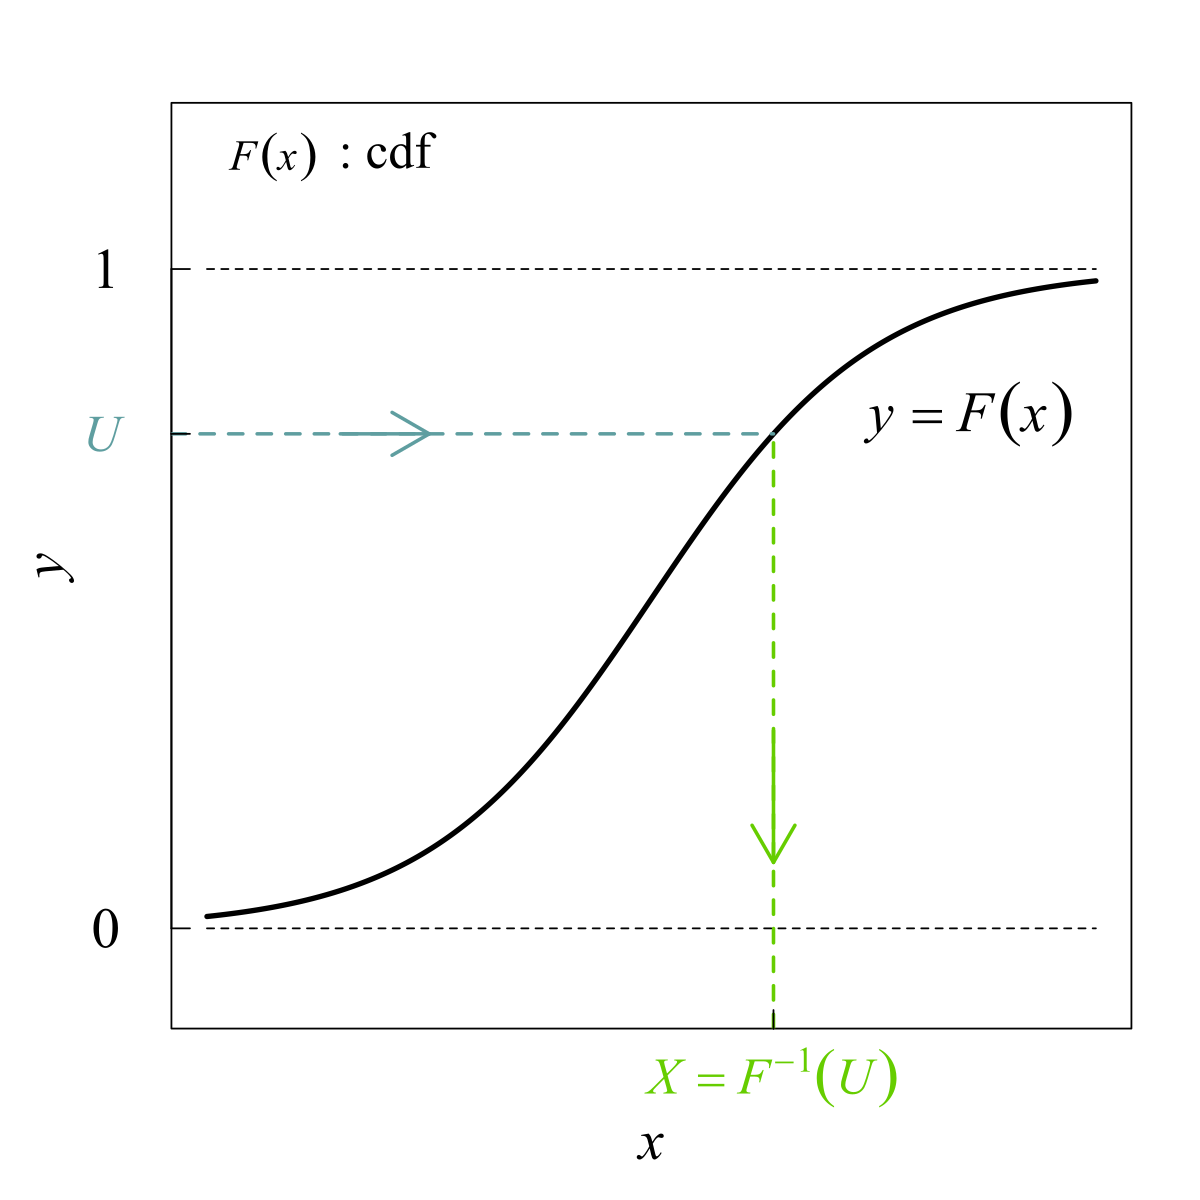
\includegraphics[width=6cm]{images/transf_inv.png}
        \caption{Método de la transformada inversa}
        \label{fig:my_label}
    \end{figure}    
\end{frame}

\begin{frame}{Método de la transformada inversa}{Distribución uniforme}
    \begin{itemize}
        \item La función de probabilidad acumulada de la distribución uniforme
        \begin{equation*}
            F(x)=\left\{\begin{array}{cc}
                 0 & x < a \\
                 \frac{x-a}{b-a} & a \leq x \leq b \\
                 1 & x > b
            \end{array}\right.
        \end{equation*}
        \item Aplicando la transformada inversa y despejando se tiene el generador \begin{equation*}
            X=(b-a)R+a
        \end{equation*}
    \end{itemize}
\end{frame}

\begin{frame}{Método de la transformada inversa}{Distribución exponencial}
    \begin{itemize}
        \item La función de probabilidad acumulada de la distribución exponencial
        \begin{equation*}
            F(x)=\left\{\begin{array}{cc}
                 1-e^{-\lambda x} & x \geq 0  \\
                 0 & x < 0
            \end{array}\right.
        \end{equation*}
        \item Al aplicar la transformada inversa y despejando se tiene el generador \begin{equation*}
            X=\frac{-\ln{(1-R)}}{\lambda}
        \end{equation*}
    \end{itemize}
\end{frame}

\begin{frame}{Método de la transformada inversa}{Distribución triangular}
    \begin{itemize}
        \item La función de probabilidad acumulada de la distribución triangular $\left[a,m,b\right]$ está dada por
        \begin{equation*}
            F(x)=\left\{\begin{array}{ll}
                 0 & x < a  \\
                 \frac{\left(x-a\right)^2}{\left(b-a\right)\left(m-a\right)} & a\leq x\leq m \\ 
                 1-\frac{\left(b-x\right)^2}{\left(b-a\right)\left(b-m\right)} & m\leq x\leq b \\ 
                 1 & b<x
            \end{array}\right.
        \end{equation*}
    \end{itemize}
\end{frame}

\begin{frame}{Método de la transformada inversa}{Distribución triangular}
    \begin{itemize}
        \item Note que si $X \sim TRIA\left(0,\frac{m-a}{b-a},1\right)$, entonces \begin{equation*}
            X'=a+(b-a)X \sim TRIA\left(a,m,b\right) 
        \end{equation*}
        \item El generador para $X$ se puede obtener a partir de la transformada inversa como
        \begin{equation*}
            X=\left\{\begin{array}{ll}
            \sqrt{m'R} & 0 \leq R \leq m'\\
            1-\sqrt{\left(1-m'\right)\left(1-R\right)} & m'<R\leq 1
            \end{array}\right.
        \end{equation*}
        donde $m'=\frac{m-a}{b-a}$
    \end{itemize}
\end{frame}

\begin{frame}{Método de la transformada inversa}{Distribuciones discretas}
    \begin{itemize}
        \item Suponga que se quiere generar una variable aleatoria discreta con función de probabilidad de masa:
    \begin{equation*}
        P\left\{X=x_j\right\}=p_j, ~ j=0,1,\dots , ~\sum_j{p_j}=1
    \end{equation*}
    \item El algoritmo a emplear es:
    \begin{enumerate}
        \item Genere un número aleatorio $R$
        \item Si $R<p_0$ entonces $X=x_0$ y pare
        \item Si $R<p_0+p_1$ entonces $X=x_1$ y pare
        \item Si $R<p_0+p_1+p_2$ entonces $X=x_2$ y pare
        \item $\vdots$
    \end{enumerate}
    \end{itemize}
\end{frame}
    
    \section{Convolución}

\begin{frame}{Método de convolución}
    \begin{itemize}
        \item La función de distribución de probabilidad de la suma de dos o más variables aleatorias independientes se conoce como \textit{convolución} de las funciones de distribución de probailidades de las variables originales.
        \item Este método de generación se aplica cuando la variable aleatoria $X$ se puede expresar como la suma de $n$ variables aleatorias que se pueden generar más fácilmente.%: $X=Y_1+Y_2+\cdots+Y_n$.
        
        %\item Las variables aleatorias de cuatro de las distribuciones más conocidas (Erlang, normal, binomial y de Poisson) pueden generarse a través de este método.
    \end{itemize}
\end{frame}

\begin{frame}{Método de convolución}{Distribución $k$-Erlang}
    \begin{itemize}
        \item La suma de $k$ variables independientes distribuidas exponencialmente, cada una con media $\frac{1}{k\theta}$ sigue una distribución $k$-Erlang con media $\frac{1}{\theta}$.
        \item Usando el método de convolución, una variable aleatoria $k$-Erlang se puede crear generando $X_1, X_2, \dots , X_k$ como variables exponenciales exponenciales y luego sumarlas para obtener $X$.
        \begin{equation*}
            X=\sum_{i=1}^{k} X_i = \sum_{i=1}^{k}{\frac{-\ln{ (R_i)}}{k\theta}}=-\frac{1}{k \theta} \ln{\left(\Pi_{i=1}^{k}{R_i}\right)}
        \end{equation*}
    \end{itemize}
\end{frame}
    
    %\section{Composición}

\begin{frame}{Método de composición}
    \begin{itemize}
        \item  Este método permite generar variables aleatorias cuando éstas provienen de una función de densidad $f(x)$ que puede expresarse como la combinación convexa de $m$ distribuciones de probabilidad $f_i(x)$.
        \item Entonces, la combinación convexa se puede expresar como: \begin{equation*}
            f(x)=\sum_{i=1}^{m}{f_i(x)I_A(x)}
        \end{equation*} donde
        \begin{equation*}
            I_A(x)=\left\{\begin{array}{cc}
                1 & \text{ si } x \in A\\
                0 & \text{ si } x \notin A
            \end{array}\right.
        \end{equation*}
        %\item Algunas de las distribuciones que se pueden expresar como una combinación convexa son: la triangular, la de Laplace y la trapezoidal.
    \end{itemize} 
\end{frame}

\begin{frame}{Método de composición}{Distribución triangular}
    
\end{frame}
    
    \section{Aceptación y rechazo}

\begin{frame}{Método de aceptación y rechazo}
    \begin{itemize}
        \item Suponga que se tiene un método eficiente para simular una V.A. con función de densidad $r(x)$ tal que $t(x)=c*r(x)>f(x)$ para cualquier valor de $x$.
        \item Podemos utilizarla para simular una distribución con función de densidad $f(x)$ mediante el siguiente algoritmo:
        \begin{enumerate}
            \item Genere $x$ con densidad $r(x)$.
            \item Genere $y$ uniforme $[0,t(x)]$.
            \item Si $y\leq f(x)$, devuelva $x$, de lo contrario vuelva al paso 1.
        \end{enumerate}
    \end{itemize}
\end{frame}

\begin{frame}{Método de aceptación y rechazo}{Distribución de Poisson}
    \begin{itemize}
        \item La función de probabilidad $P(X=x)=\frac{e^{-\lambda}\lambda^x}{x!}$ para $x\geq 0$.
        \item El procedimiento para generar una V.A. Poisson $N$ con parámetro $\lambda$, es el siguiente:
        \begin{enumerate}
            \item Sea $n=0$, $P=1$.
            \item Genere un número aleatorio $R_{n+1}$ y reemplace $P$ por $P*R_{n+1}$.
            \item Si $P<e^{-\lambda}$, entonces acepte $N=n$, de lo contrario, rechace el $n$ actual, incremente $n$ en uno y regrese al paso 2.
        \end{enumerate}
    \end{itemize}
\end{frame}
    
    \section{Distribución normal}

\begin{frame}{Distribución normal}
    \begin{itemize}
        %\item Muchos métodos se han desarrollado para generar variables aleatorias normalmente distribuidas.
        \item El método de la transformada inversa no puede ser aplicado fácilmente porque la función de distribución acumulada para una variable aleatoria con distribución normal no puede ser escrita en forma cerrada.
        \item La función de distribución acumulada de la distribución normal está dada por:
        \begin{equation*}
            \Phi (x) = \int_{-\infty}^{x} \frac{1}{\sqrt{2\pi}} e^{-\frac{t^2}{2}}dt, \quad -\infty<x<\infty
        \end{equation*}
    \end{itemize}
\end{frame}

\begin{frame}{Distribución normal}{Aproximación al Teorema del límite central}
    \begin{itemize}
        %\item Aplica el teorema del límite central en variables aleatorias $r\sim U(0,1)$.
        \item Si $R_1, R_2, \dots, R_n \sim UNIF(0,1)$, entonces \begin{equation*}
            Z=\frac{\sum {R_i} - \frac{n}{2}}{\sqrt{\frac{n}{12}}}
        \end{equation*}
        sigue aproximadamente una distribución normal estándar. 
        \item Con $n=12$ se obtiene la forma:
        \begin{equation*}
            Z=\sum r_i - 6
        \end{equation*}
        %\item Este método requiere 12 números aleatorios independientes para generar un solo número aleatorio normal.
    \end{itemize}
\end{frame}

\begin{frame}{Distribución normal}{Método de Box-Muller}
    %\begin{itemize}
        %\item Este método genera dos variables aleatorias de una distribución normal estándar y requiere dos números aleatorios uniformes entre 0 y 1:
        \begin{enumerate}
            \item Genere dos números aleatorios independientes $R_1$ y $R_2$  de una distribución $UNIF(0,1)$.
            \item Devuelva \begin{equation*}
                Z_1=\sqrt{-2 \ln{R_1}} \cos{\left(2\pi R_2\right)}
            \end{equation*} y \begin{equation*}
                Z_2=\sqrt{-2 \ln{R_1}} \sen{\left(2\pi R_2\right)}
            \end{equation*}
        \end{enumerate}
        %\item Desafortunadamente el método no es eficiente pues requiere computar las funciones trigonométricas seno y coseno.
    %\end{itemize}
\end{frame}

\begin{frame}{Distribución normal}{Método Polar}
    %\item Es un método alternativo al algoritmo de Box-Muller, pero no necesita funciones trigonométricas:
    \begin{enumerate}
        \item Genere dos números aleatorios independientes $R_1$ y $R_2$ de una distribución $UNIF(0,1)$.
        \item Defina $V_1=2R_1 - 1$,  $V_2=2R_2 -1$ y $S=V_1^2+V_2^2$.
        \item Si $S>1$ vuelva al paso 1, de lo contrario devuelva \begin{equation*}
            Z_1=\sqrt{\frac{-2 \ln{S}}{S}}V_1
        \end{equation*} y \begin{equation*}
            Z_2=\sqrt{\frac{-2 \ln{S}}{S}}V_2
        \end{equation*}
    \end{enumerate}
\end{frame}

\begin{frame}{Distribución normal}{Método de Inversión de Rao, Boiroju y Reddy}
    \begin{itemize}
        \item Emplea un ajuste logístico de la función de distribución acumulada de la distribución normal estándar, dado por:
        \begin{equation*}
            \Phi (Z)=\frac{1}{1+e^{-[1.702 Z]}}
        \end{equation*}
        \item Usa esta relación como una aproximación para utilizar luego el método de la transformada inversa con el siguiente algoritmo:
        \begin{enumerate}
            \item Genere un aleatorio $R\sim UNIF(0,1)$.
            \item Devuelva \begin{equation*}
                Z=\frac{-\ln{\left(\frac{1}{R}-1\right)}}{1.702}
            \end{equation*}
        \end{enumerate}
    \end{itemize}    
\end{frame}
    
    \nocite{dunna}
    \nocite{BCN}
    \nocite{PSD}
    \nocite{ross}
    \section*{Referencias} %You can remove this if you do not want to use it
        \begin{frame}{Referencias}
            \printbibliography
        \end{frame}
     
    \section{}   
        \begin{frame}{}
            \begin{figure}
                \centering
                
\includegraphics[width=6cm]{images/model.png}
                %\caption{Caption}
                %\label{fig:my_label}
            \end{figure}
        \end{frame}

\end{document}
